\chapter{Structrual Variant Detection in Single Cells}
\label{sec:mosaicatcher}

Here, I present the current state of a project with the objective to develop a
computational method for \sv detection in Strand-seq data. This method is being
developed together with \jan and \ashley as well as with our collaborators
\david, \maryam, and \marschall from the Max-Planck Institute for Informatics,
Saarbrücken. \ashley and \jan conceived the general concept of \sv discovery
based on the signals provided by Strand-seq data. \marschall and \david
contributed analyses related to phasing, general improvements to the overall
work flow and fruitful discussion on many aspects. \maryam developed the
Bayesian classification approach described below. Also work from \venla on
\acl{sce} events was included into this method.
The main implementation and all other analyses, including figures, are my own.
At last, I would like to thank \balca, who provided the cell lines utilized for
demonstration purposes, and \landsdorp's lab, who carried out the Strand-seq
experiments on these cell lines.





\section{Structural variants in the context of somatic mosaicism}
\label{sec:mosaic_mosaicism}

As briefly introduced earlier, somatic mosaicism refers to the presence of
genetically distinct subpopulations of cells within an individual
\citep{Youssoufian2002}. The relatively high susceptibility of dividing to mutagenesis
suggests that nearly all of the cells in our body harbor variation, ranging from \acp{snv}
to large \acp{sv} \citep{Campbell2015}. Fortunately, the majority of these
accumulated variants do not affect our health. Certain cases of somatic mosaicism are even
part of our physiological development, such as the programmed rearrangements of
T-cell receptor genes the tendency of liver cells to develop polyploidy
\citep{Forsberg2017,Davoli2011}. However, mosaicism has also been linked to
disease and it is becoming increasingly clear that \aclp{sv} play an important
role in this process \citep{Forsberg2017}. The prime example is cancer, which
arises from the clonal expansion of a cell that carries beneficial (driver)
mutations as well as passenger mutations \citep{Forsberg2017}. But other
diseases, such as type 2 diabetes mellitus or Alzheimer, have been linked to the
presence of mosaic mutation, too \citep{Forsberg2017}. Moreover, the amount of
mosaicism has been shown to increase with age. For example, \citet{Forsberg2012}
observed Meagabase-range aberrations in people at the age of 60 and above, but not in
younger subjects. Especially the blood compartment, but also skin, appear to be
affected by somatic mutation---as, for instance, was shown in the blood of a
115-year old woman, which harbored a manifold-higher amount of mosaic variants
than other tissues \citep{Forsberg2017,Holstege2014}.

Single-cell studies have uncovered vast amounts of somatic copy number
alterations in cancer \citep{Navin2011,Demeulemeester2016}. They also revealed
unforeseen amounts of somatic mosaicism in brain tissue, including in
post-mitotic neurons, which were analyzed on the level of \acp{snv}, \acp{cnv}
\acp{mei} \citep{Lodato2015,Cai2014,Evrony2012}.
These single-cell methods typically rely on \explain{whole-genome amplification}{
    Method to amplify the entire DNA in a nucleus prior to single-cell sequencing.
    Multiple technologies were put forward for this task, such as MDA or MALBAC
    \citep{Dean2002,Zong2012}, witch have been compared recently for their
    usability in \cnv detection \citep{Deleye2017}}
to increase the amount of DNA available for sequencing. However, the amplification step has been noted to
introduce biases that hamper detection of \acp{cnv} below several Megabases in
size \citep{Deleye2017}. While single-cell \cnv detection has been
constantly improving since, allowing much higher resolution
\citep{Garvin2015,Gao2016,Bakker2016,Knouse2016}, the detection of copy-neutral \acp{sv} has
been lagging behind.

These limitations made it difficult to robustly discern structural variation,
especially copy number-neutral and complex events in the context of cellular
heterogeneity. Consequently, the role of somatic \acp{sv} remains comparatively
underexplored to other forms of genetic variation. In this chapter, I present a
fully novel way to study \acp{sv} on the single-cell level. Based on the
single-cell sequencing method Strand-seq, we developed a computational approach
for the detection of previously difficult-to-ascertain \sv classes. Below, I
explain this method in detail and give an outlook on the future research that
can and will be done using this new approach.






\section{\textsc{Mosaicatcher}: A novel method for single-cell SV detection}
\label{sec:mosaic_mc}

Strand-seq generates sequencing reads that are all of the same directionality
when they stem from the same homologue. As explained in \cref{sec:strandseq},
this is achieved by labeling and degrading the non-template strand of
actively replicating cells. When the resulting sequencing reads are mapped to a
reference assembly, they map either to the Watson (W) or Crick (C) strand. The
presence of two homologous chromosomes then leads to the presence WW, CC, or WC
chromosomes, which I call their \emph{inherited strand states}.
Here, I show how these unique characteristics of Strand-seq reveal the presence
of seven different \sv classes and demonstrate our computational method called
\mc that implements this idea.

%\afterpage{%
%    \clearpage%
%    \ifodd\value{page} \expandafter\afterpage \fi {%
    \begin{figure}[t!]                                             % cell BM160815_WT_007p1 from BM160815_WT.200000.pdf
        \captionsetup{type=figure}
        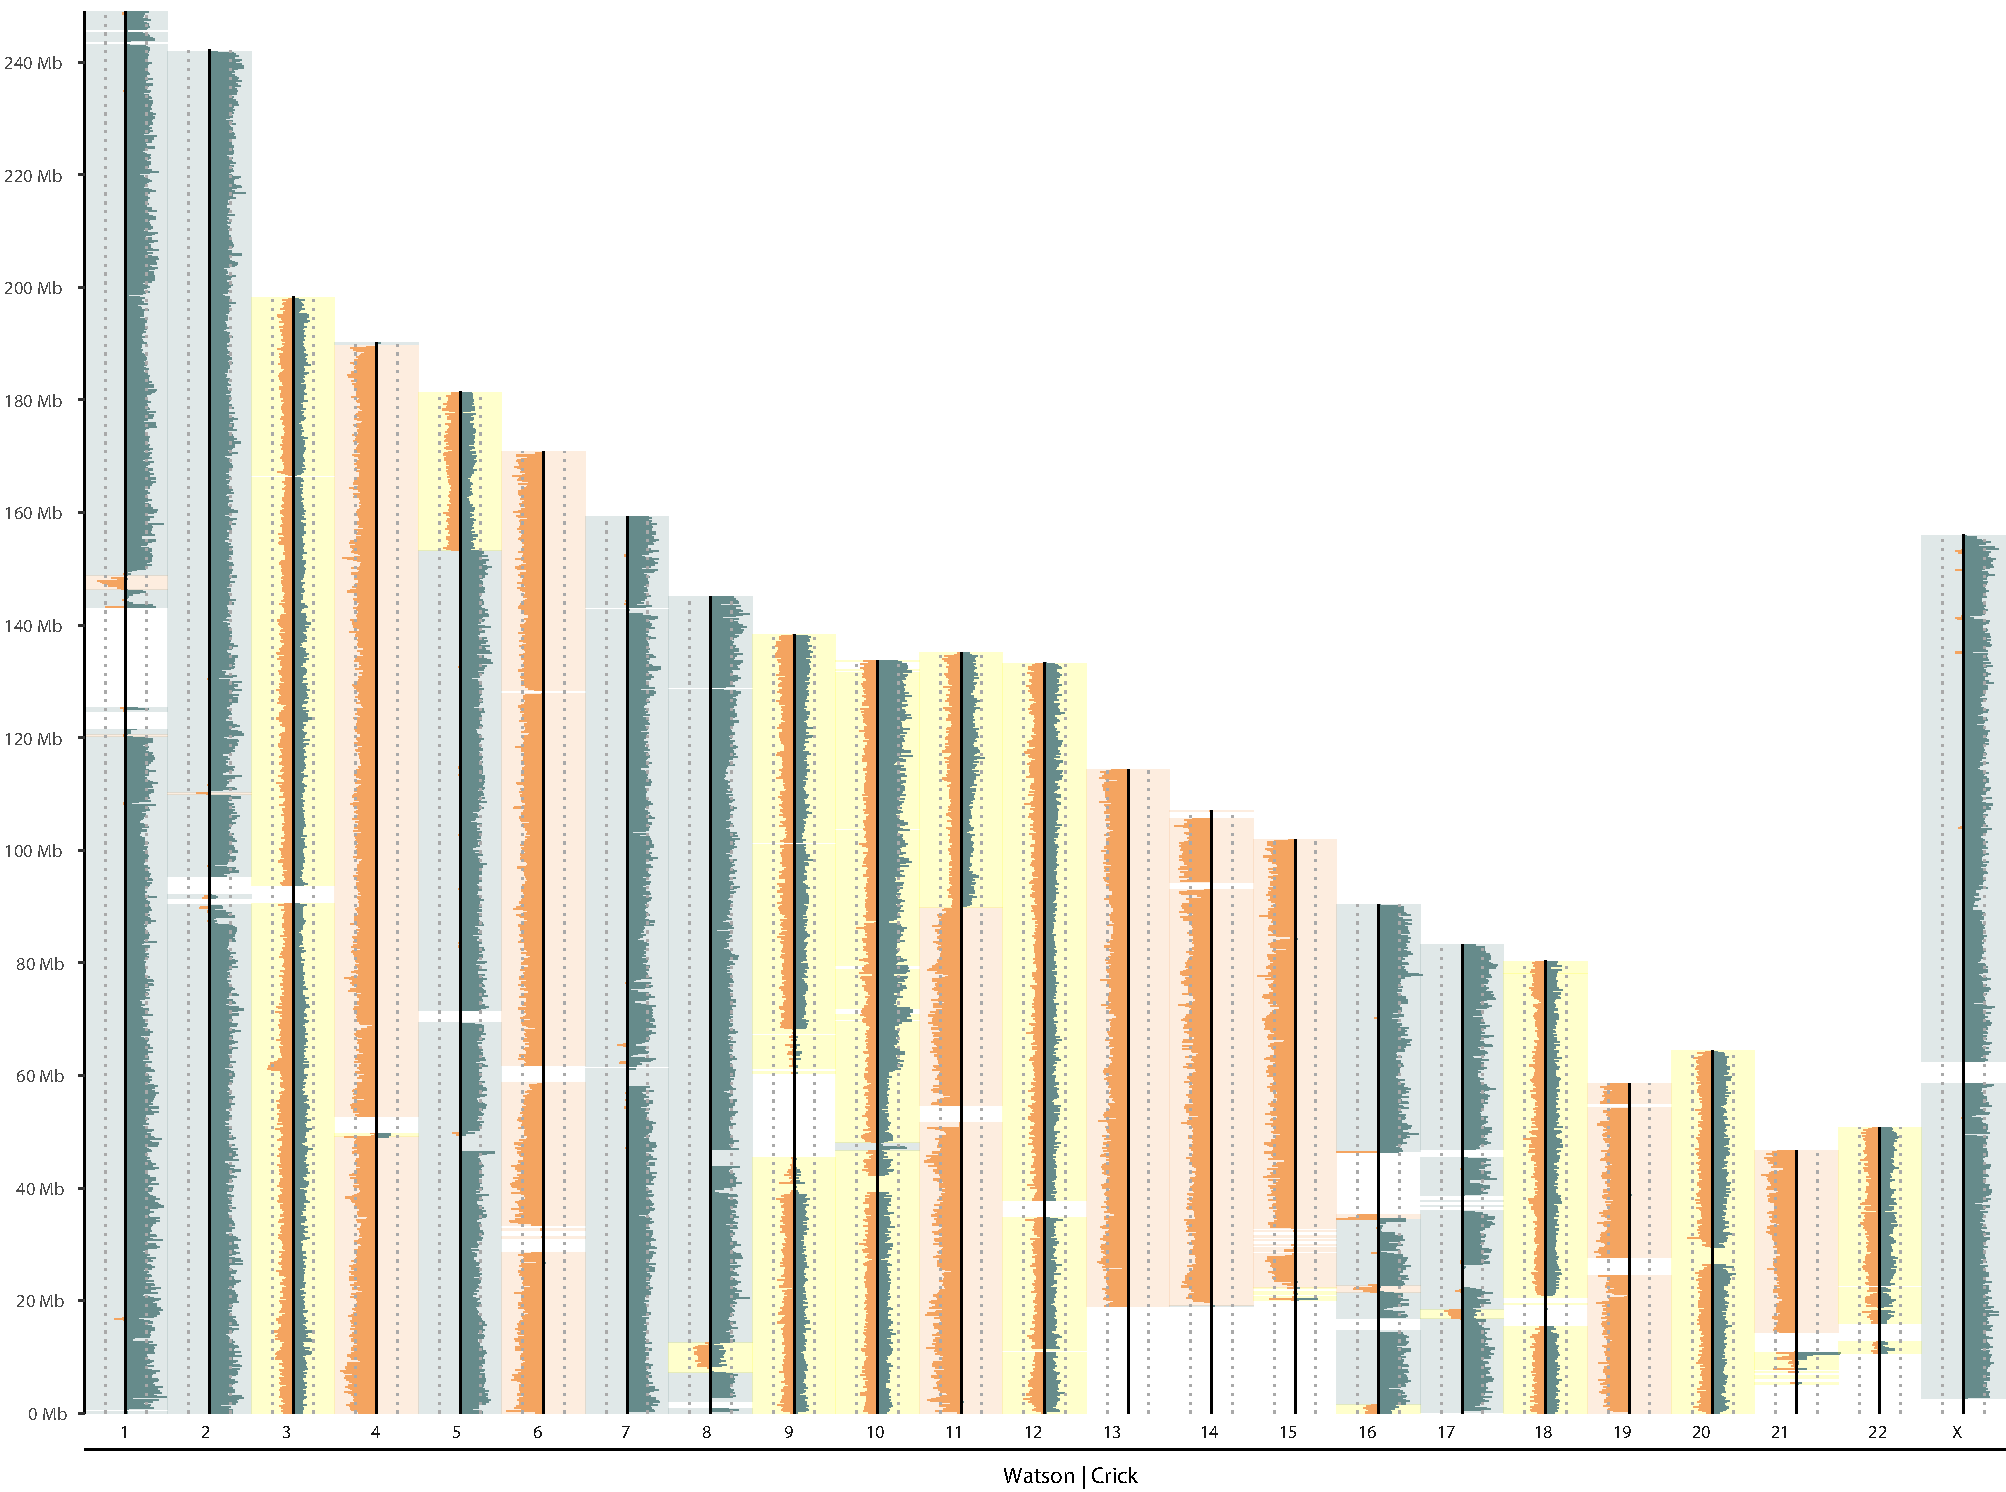
\includegraphics[width=\textplusmargin,inner]{ss_lib_rpewt.pdf}
        \figcap{ss_library}{Example of a single cell Strand-seq library}{
            Here, a single cell Strand-seq library of an \rpe-I wild type cell
            line is displayed using the plot function of \mc.
            Each vertical panel shows binned read counts of one chromosome, with
            the Watson strand on the left, in orange, and the Crick strand on
            the right, in blue. In the cell shown here, each 200~kb-bin contains
            a median of 76 total reads, which is depicted by
            dotted lines. Some regions, e.g. the centromere of chromosome 1 or
            the sub-telomeric regions of chromosomes 13--15, are not coverded by
            reads because of mappability issues; these bins are excluded from
            further analyses. The estimated strand inheritance state of each bin
            is color-coded in the background: blue for CC, orange for WW and yellow
            for WC. Chromosomes 5 and 11 carry \acp{sce}, which are visible by a
            change in the strand inheritance state that continues to the end of
            the chromosomes.}%
    \end{figure}
%    }}

\Cref{fig:ss_library} depicts Strand-seq data from a single cell of an \acf{rpe}
wild type cell line (courtesy by \balca and \landsdorp). This cell-wide overview
plot was generated using \mc and is typically the starting point for
an analysis of Strand-seq data. The procedure leading to this plot is outlined
briefly in \cref{sec:mosaic_method}.

These overview plot allows an initial judgment on the success, quality, and depth
of a Strand-seq library. In the cell shown here, reads aligning to either W or C
strand were binned at 200~kb resolution. The cell was sequenced at ample depth
(median of 76 reads per bin), shows the Strand-seq characteristic strand
inheritance patterns (WW, CC, and WC chromosomes) and is of high quality, which
can be judged from the low number of reads on the opposite strand in WW or CC
cells and a fairly even coverage distribution. Experimental parameters
influencing the quality of Strand-seq libraries are discussed in detail by
\citet{Sanders2017}.

\Cref{fig:ss_library} further gives a first impression of genomic rearrangements
in this cell. For example, the region of WW reads at around 120~Mb on chromosome
1 reveals an inversion of this locus in respect to the reference assembly. The
most prominent alterations are visible on chromosomes 5 and 11, though. Here,
the strand inheritance states change at one position (specifically,
at 155~Mb on 5 and 90~Mb on 11) and remain consistent to
the end of the chromosome from there. These positions mark \emph{\acf{sce}} events,
which are reciprocal exchanges between two identical sister chromatids and
which can be specifically measured using Strand-seq \citep{Falconer2012}.
\Acp{sce} occur randomly across the genome and must not be mistaken with other
classes of \acp{sv} for our purpose.





\subsection{Three signals within Strand-seq data are distinctive of SVs}
\label{sec:mosaic_concept}

Strand-seq libraries reveal the presence of large \Acl{sv}. This had been shown
for inversions in the past by \citet{Sanders2016}. Here, we conceptually identified seven
different \sv classes that can be revealed in Strand-seq data, five of which are
principally discernible within a single cell (deletion, duplication, inversion,
inverted duplication, and \loh), and two that become apparent across a population
of cells (aneuploidy and translocation). These \sv classes can be distinguished
using three independent signals: (1) the normalized read coverage of a locus,
which corresponds to a diploid state (2N) in a non-affected locus.
(2) The strand ratio, i.e. the number of W reads over the number of C reads.
Alternatively, a fraction can be used here, for example the Watson fraction
W/(W+C). (3) Haplotype information. When whole-chromosome haplotypes are known
at sites of \acp{snv}, sequencing reads overlapping such variants can be queried for
both their original homologue \emph{and} their strand direction.
These alleles can be used to reason about potential rearrangements. In the
following report, I refere to the two homologues (or their haplotypes) as $h_1$
and $h_2$
Below I explain how we can utilize the combination of these signals to detect,
genotype and phase the seven \sv classes. \Cref{fig:mosaic_examples} contains examples of
five different \sv classes that we identified in \rpe cell lines.

\FloatBarrier
\begin{table}[t]%
\newcommand\ccb{\cellcolor{blue!15}}
\newcommand\cco{\cellcolor{orange!15}}
    \begin{adjustbox}{width=\textplusmargin,inner}%
    \begin{tabu} to \textplusmargin {X[l] c c c c l c c c c}
        \toprule
          & \multicolumn4{c}{WC chromosome} & & \multicolumn4{c}{WW chromosome} \\
         \cmidrule{2-5} \cmidrule{7-10}
          & & & \multicolumn2{c}{Haplotype} & & & & \multicolumn2{c}{Haplotype} \\
        \cmidrule(lr){4-5} \cmidrule(lr){9-10}
         & Cov. & W.f. & \emph{W} & \emph{C} & & Cov. & W.f. & \emph W & \emph{C} \\
        \midrule
        Reference allele             &      2N &      50\% & $h_1$   & $h_2$     & &      2N &      100\% & $h_1 + h_2$     & - \\
        Deletion of $h_1$            &      1N &       0\% & -       & $h_2$     & & \ccb 1N & \ccb 100\% & $h_2$           & - \\
        Deletion (homozygous)        &      0N &         - & -       & -         & &      0N &          - & -               & - \\
        Duplication of $h_1$         &      3N &      66\% & $2 h_1$ & $h_2$     & & \ccb 3N & \ccb 100\% & $2 h_1 + h_2$   & - \\
        Duplication (homozygous)     &      4N &      50\% & $2 h_1$ & $2 h_2$   & &      4N &      100\% & $2 h_1 + 2 h_2$ & - \\
        Inversion of $h_1$           &      2N &       0\% & -     & $h_1 + h_2$ & & \ccb 2N & \ccb  50\% & $h_2$ & $h_1$       \\
        Inversion (homozygous)       & \cco 2N & \cco 50\% & $h_2$   & $h_1$     & &      2N &        0\% & -     & $h_1 + h_2$ \\
        Inverted duplication ($h_1$) & \cco 3N & \cco 33\% & $h_1$ & $h_1 + h_2$ & & \ccb 3N & \ccb  66\% & $h_1 + h_2$ & $h_1$ \\
        \bottomrule
    \end{tabu}
    \end{adjustbox}
    \tabcap{mosaic_sv_signals}{Distinct signatures of focal SVs in Strand-seq
    data}{SVs can be identified based on three separate signatures of Strand-seq
    data: the total read coverage (\emph{Cov.}), the strand ratio (here shown
    as Watson fraction; \emph{W.f.}), and the presenece of haplotype-tagging
    \acp{snv} on each strand (\emph{Haplotpye}). The table shows how
    focal \sv types can be inferred from these signals. This is different
    for WC chromosomes than for WW or CC chromosomes. For the sake of simpliciy,
    the table only shows the WW case and assumes heterozygous variants to affect
    haplotype $h_1$. Entries in orange are \sv classes that cannot be
    distinguished unambigously using only coverage and Watson fraction.
    Specifically, a homozygous inversions remain hidden in WC cells and an
    inverted duplication of $h_1$ cannot be distinguished from a duplication of
    $h_2$. Entries marked in blue cannot be phased based on coverage and Watson
    fraction alone. However, all these cases can be disentangled when
    haplotype-resolved \acp{snv} are available or by integrating information
    across several cells that share an \sv.}
\end{table}

\paragraph{Deletions and duplications}
\Acp{cnv} alter the total read coverage of an affected locus. A deletion
decreases the coverage from 2N to 1N, i.e. by a factor of two, and is hence
typically easier to detect than higher copy number states---the same has been observed for other read
depth-based \sv callers. Duplications, which increase copy number to 3N, alter
the read depth only by a factor of 1.5 compared to the reference state.
Homozygous duplications increase the copy number even to 4N. Homozygous
deletions are marked by a complete absence of reads---they thus provide the
strongest change in read depth, with the only caveat that they resemble regions
of low mappability such as the centromere on chromosome 1. Homozygous deletions
are hence best studied in the presence of a control sample not carrying
the deletion.

In contrast to classic read depth analysis, Strand-seq additionally provides
strand information. For example, a heterozygous deletion in a WC chromosome will
only lack reads on one of the strands. Similarly, a heterozygous duplication
will increase coverage only on one strand. In a WW or CC cell, strand
information does not add supportive evidence, but when phased \acp{snv} are
available, only one homologue will be deleted/duplicated.
\Cref{tab:mosaic_sv_signals} summarizes in detail how these signals
allow to differentiate the focal \sv classes that I cover here.

\paragraph{Copy-neutral variants}
Inversions do not change copy number, but become visible as a change in strand
ratio. A heterozygous inversion in a WW cell, for example, switches the observed strand
state to WC within the inverted locus. In a WC cell, it becomes WW or CC. Again,
in the WC cell the inversion can be phased trivially based on strand
directionality, whereas in the WW or CC case further \snv information has to be
consulted for phasing. A homozygous inversion is a special case: It changes a WW
chromosome into CC, making the locus clearly stand out, but it cannot be
observed within a WC cell. This is because both alleles change their strand
state, leading again to a WC region. This case can be disentangled with the help
of phased \acp{snv} (\cref{tab:mosaic_sv_signals}).

Another copy-neutral \sv is class \loh. In a \loh event, one homologue is
``overwritten'' by the other homologue, leading to extended regions of
homozygousity. To reveal \loh, the alleles of \acp{snv} must be assessed. We recently
noted sporadic regions of \loh within cells of a lymphoblastoid cell
line (data not shown). This analysis as well as other work on haplotype information
was spearheaded by \david and will hence not be covered in this
dissertation.

\paragraph{Complex variants}
Complex variants can partly be discovered in Strand-seq data, too. We chose
inverted duplications as a particular candidate, as this class has been found to
be abundant both on the small (\cref{sec:balancer}) as well as on the large
scale \citep{Chaisson2017}. As \cref{tab:mosaic_sv_signals} shows, inverted
duplications are marked by an increase in copy number as well as a flip in
strand orientation. In a WC cell, such an event cannot be distinguished from a
normal duplication unless haplotype information is available. \Cref{fig:mosaic_examples}
includes an example of an inverted duplication within \rpe wild type cells.

\figuretextplusmargin[t!]{mosaic_sv_examples.pdf}{mosaic_examples}{Examples of SVs
    in RPE cells}{Strand-specific count data in 100~kb bins (Watson orange,
    Crick blue) are shown in several chromosomal regions of \rpe cells.
    \subpanel{A} Four loci harboring \acp{sv} are shown across three cells each.
    The affected
    loci (marked by dashed lines) show the characteristic changes in read
    coverage and strand state that were described in \cref{tab:mosaic_sv_signals}.
    \subpanel{B} A copy number gain of the q-arm of chromosome 10 is visible. The
    strand state of the extra copy correlates with the strand inheritance
    pattern of chromosome X (same cells for both chromosomes shown). This
    observation is best explained by an imbalanced translocation, as shown in
    the schematic to the right.
    \subpanel{C} Five chromosomes of cells from the tetraploid RPE C29 cell line
    (courtesy by \balca and \landsdorp) were selected to represent the five
    possible strand inheritance patterns in a tetraploid cell: WWWW, WWWC, WWCC,
    WCCC, and CCCC.}


\paragraph{Aneuploidy}
In a Strand-seq experiment, each homologue of a chromosome is sequenced in
either W or C orientation. This fundamental property remains valid even in the
presence of more than two homologues. In a tetraploid cell, for example, a
chromosome is inherited in any one of five states: WWWW, WWWC, WWCC, WCCC, or
CCCC. By looking across a population of cells, Strand-seq can disclose the
ploidy of each chromosome, assuming it is not heterogeneous
(\cref{fig:mosaic_examples}). A
usual way to estimate ploidy from \mps data is to assess the \baf of \acp{snv} within a bulk
sample---in a tetraploid chromosome, some \acp{snv} will be present at ratios of
25 or 75\%. Interestingly, Strand-seq detects ploidy even in the complete
absence of homologue-speicific variants, for example in cells with multiple
copies of the same homologue such as the CHM1 cell line \citep{Steinberg2014}.
To the best of our knowledge, this cannot be achieved by any other method.

\paragraph{Translocations}
At last, also translocations can be revealed using Strand-seq.  A reciprocal
translocation alters the strand inheritance state of two chromosomes
simultaneously: An exchange between a WW and a CC chromosome, for instance, would switch the
strand inheritance pattern to WC in both these chromosomes. However, such
changes in strand state can initially not be distinguished from randomly
occurring \sce events. However, a strong correlation of strand state changes
between two chromosomes is indicative of a traslocation event. In the \rpe wild
type cell line (\cref{fig:mosaic_examples}), we report an \emph{imbalanced}
translocation between chromosomes 10 and X, which had been noted
beforehand\footnote{In the description of the commercially available
    ``hTERT RPE-1'' cell line, a derivative of X is recognized, but chromosome
    10 is not mentioned. Source: \url{https://www.lgcstandards-atcc.org/Products/All/CRL-4000.aspx}}.
Here, chromosome 10 shows an increase in copy number on the q-arm that seems not
to be consistently in the same strand across cells. However, the strand
inheritance state of the extra copy perfectly matches the strand inheritance
pattern of chromosome X. This suggests that the extra copy of chromosome 10 is
linked physically to chromosome X. By correlating strand states across
chromosomes in this way, translocations can be discovered. The very same idea
has been used to assign unmapped contigs of the reference assembly to
chromosomes \citep{Hills2013}.







\FloatBarrier
\subsection{Automated SV detection}
\label{sec:mosaic_method}

In order to capture this spectrum of \sv classes, my collaborators and I
designed a computational approach for \sv calling from Strand-seq data.
This approach is implemented in a tool called \mc, which is currently being
developed. The core principle consists of the three steps (1) binning, (2)
segmentation, and (3) classification and is explained below. My code for the
first two steps is available online at
\url{https://github.com/friendsofstrandseq/mosaicatcher}.
The third part is being maintained by \maryam and can be found at
\url{https://github.com/friendsofstrandseq/MaRyam}. At last, the combined
workflow is available at \url{https://github.com/friendsofstrandseq/pipeline}.

\paragraph{Binning}
Strand-seq data is extremely sparse: the best libraries currently produced
contain around 300 reads per Megabases \citep{Chaisson2017,Sanders2017}. In
order to work with sparse data, I applied a binning scheme that summarizes
sequencing reads in windows of a given size, e.g. 50~kb. Alternatively, these
bins can have variable sizes (dynamic-width bins) to accommodate for regions of
low mappability. The transformation to binned counts allowed us to apply a
statistical model to estimate the expected number of reads per
bin---specifically, we utilized a \nb distribution, as I describe
later. Prior to binning, sequencing reads are filtered for low mapping quality
(by default, a minimum score of 10), supplementary alignments, and \pcr duplicates.
Moreover, I only each read pair was counted only once to avoid double-counting of
sequenced fragments. I utilized the \htslib library within my implementation
to efficiently read and filter sequencing data.

Given the strand-specific binned counts, I implemented a plot function to
generate overview plots as shown in \cref{fig:ss_library}. At first, bins that
consistently appear as outliers in all cells are masked: this is typically the
case in centromeric or telomeric regions with zero read coverage. Further, I designed a classifier to
distinguish WW, WC, and CC states of each bin. This classifier is supposed to
tell the class of each bin based on its strand-specific read counts, but it
should also smoothen out fluctuations in single bins.
To achieve this, I implemented a \hmm with a multivariate \nb
emission distribution. The transition probability of the \hmm is chosen
according the expected number of \acp{sce} within a cell (e.g. 10 transitions
across all chromosomes). Its output is used as background color in
aforementioned overview plots and guides a researcher in detecting \acp{sce} and
other rearrangements in a single cell.

\paragraph{Segmentation}
The second step towards \sv calling is to detect the boundaries of potential
\acp{sv}. This had been done in the past by merging data of all cells in a
strand-aware fashion and detecting boundaries within the merged signal
\citep{Sanders2016}. However, this approach has the disadvantage that it can
mask subclonal variants, especially the ones at low allele frequency that we
are particularly interested in. Boundaries have also been determined within
single cells separately, e.g. based on a \hmm similar to our aforementioned approach \citep{Bakker2016}. However, this
leads to the subsequent challenge of forming consensus boundaries across all
cells. Instead, I explored multivariate segmentation algorithms that consider
all cells simultaneously, yet still recognize them as individual cells. This is
further elaborated in \cref{sec:mosaic_segmentation}. Notably, the segmentation
algorithm is expected to provide potential \sv breakpoints, which are then
tested in the subsequent step. In order increase sensitivity, we thus allow the
segmentation to predict slightly too many boundaries that we resolve in a subsequent step.

\figurearbitrary[t!]{0.5}{mosaic_rpe_mean_var.pdf}{mean_var}{Mean variance
    relationship of binned read counts}{Each dot represents one cell of the
    \rpe-1 wild type cell line. Shown here are the mean number of reads per
    200~kb-bin vs. their variance. In a theoretical \nb distribution, mean and
    variance show a perfectly linear relationship with a slope $p$. In real data,
    we estimate $p$ by fitting a line without intercept.}

\paragraph{Classification} The third and final step is to test segments for the
presence of \acp{sv} (theory and implementation contributed by \maryam; figures
from me). In order to classify segments into either a \sv or non-\sv state, we
employ an elaborate Bayesian model based on \acl{nb} distributions.
Specifically, we model the read coverage in each strand by a \nb distribution,
which is adjusted to capture the expected number of reads within a given region.
Both strands combined yield a joint distribution for all possible strand
combinations, i.e. WW, WC, or CC, but also including abnormal states such as C, WWC, CCCC,
and so on. Each of these joint strand states can then be interpreted in respect
to the expected strand state in the chromosome and cell. For example, a WC state would
signify a heterozygous inversion if it occurred in a WW chromosome, but no \sv
(or a homozygous inversion!) if it occurred in a WC chromosome.
\Cref{fig:nb_examples} gives a detailed example of how read counts are modeled
in a joint \nb distribution. The dispersion parameter of the \nb distribution,
$p$, is estimated across all cells, as \cref{fig:mean_var} explains. The second
\nb parameter controls the number of expected reads within a locus and must
hence be scaled to the size of the tested region. In line with our intuition,
a \nb distribution yields a clearer separation for higher counts, i.e. in larger
genomic regions intervals than for small \acp{sv}. A shortcoming of our
approach is that the \nb distribution offers no intuitive way to model an
expectation of zero counts, i.e. the absence of reads. We hence added a factor
$\alpha \approx 5\%$ to our model to formulate a \nb distribution that captures
this case. For instance, in a WW regions with $e$ expected total reads, the
expected number of C reads would be modeled by $\alpha \cdot e$ and the expected
number of W reads by $(1-\alpha) \cdot e$. In the end, the
estimated \nb probabilities for all \sv classes are considered across cells to
make a final decision about an \sv.

\figuretextplusmargin[t!]{NB_example.pdf}{nb_examples}{Graphical example of the
    negative binomial model}{The subplots on the top left and bottom right (in
    both panels) show the probability density functions of three \nb
    distributions. These distributions describe the probability of a given
    number of reads for the possible copy number states 0N, 1N, and 2N.
    In this example, the expected number of reads in a 2N state is 20 (blue
    curves). Both strands are modeled by separate \nb distributions, that, when
    combined, yield a joint probability (area of the rectangles; top right subpanels).
    Here, only the joint states W, C, WW, WC, CC are shown for the sake of
    simplicity (other possible states would be WWW, WWC, WWCC, and so on).
    \subpanel{A} 12 W and 8 C reads were observed, for which the joint
    strand state WC is by far the most likely one. \subpanel{B} 16 W and
    4 C were observed, which are best explained by a joint WW state, yet the
    difference to the runner up (WC) is not big.
    For SV calling, these joint states have to be interpreted in respect to the
    strand inheritance state of the chromosome: for example in a WC cell,
    example \textbf{A} would be rejected (WC, i.e. reference, is the most likley
    state) but example \textbf{B} would be considered for a heterozygous inversion
    (WW state).}

\paragraph{Additional steps}
Together with \maryam, \marschall and \david, we set up an automated workflow
with the aim to process Strand-seq data all the way from raw sequencing files to
final list of \sv predictions. This pipeline, which is based on the workflow
engine \snakemake, involves many other relevant steps in addition to the
tripartite calling procedure explained above, two of which shall be mentioned
here. First of all, the dominant strand state has to be determined for each cell
and chromosome in order to guide the \sv classification. This includes the
detection of \sce events. In order to achieve this, \venla implemented a
heuristic method to estimate strand states and \acp{sce} based on the output of
the strand state \hmm of \mc. This performed well when it was tested against experts'
opinions on real-world Strand-seq data. Secondly, haplotype information must be
annotated. \david hence incorporated functionality to annotate haplotypes in WC
chromosomes based on the \strandphaser tool. Interestingly, the phasing of \acp{snv}
can be performed from Strand-seq data alone \citep{Porubsky2016}, which was also
built into the the workflow. With sufficient coverage, Strand-seq data can
even be used for \snv detection, which is a required input to phasing. Together,
this workflow supplies all input for subsequent \sv calling on Strand-seq data
without the requirement for additional data sets.






\subsection{A multivariate segmentation algorithm to find SV breakpoints}
\label{sec:mosaic_segmentation}

The objective of the segmentation step is to group the genome into consecutive regions of
the same copy number. In Strand-seq data, I apply this principle to both strands
separately. It can be formulated as a problem of placing $k$
breakpoints in such a way, that the resulting consecutive segments best
represent a single copy number state each---``best'', in this case, refers to
tge squarred (Gaussian) error, which shall be minimized. This problem gained much attention with the
availability of comparative genomic hybridization arrays to map \acp{cnv}.
Several methods were put forward for this task and a popular one is circular
binary segmentation \citep{Olshen2004,Venkatraman2007}. Today, these techniques
are also commonly applied to \mps data. The number of data points (hybridization
loci in arrays, or genomic bins in \mps experiments) critically impact the
runtime of such methods. Circular binary segmentation is efficient in this
respect, but it uses a heuristic approach (e.g. placing one breakpoint after the
other) that does not guarantee to find an optimal solution. In contrast, the
\textsc{tilingArray} \citep{Huber2006} package uses a dynamic programming
algorithm to find the optimal solution according to the squared error criterion.
As this algorithm does not scale well to deep \mps data, other approaches have
been proposed, such as the Group fused LASSO formulation \citep{Bleakley2011}.

As Strand-seq data is inherently sparse, problem size is not a limitation factor
in our application. For example with 50~kb bins, chromosome 1 still only
contains \textasciitilde5000 data points. I hence designed and implemented an
algorithm for Strand-seq segmentation that is based on the \textsc{tilingArray}
principle\footnote{Original from \url{http://bioconductor.org/packages/release/bioc/html/tilingArray.html};
    implemented independently (including major changes) in \mc (see the file
    \texttt{segmentation.hpp} at \url{https://github.com/friendsofstrandseq/mosaicatcher})}.
The \textsc{tilingArray} algorithm internally uses a cost matrix that defines
how expensive (in terms of variance) each consecutive segment is. A dynamic
programming algorithm then choses the optimal combination of breakpoints. The
calculation of the cost matrix in \textsc{tilingArray} assumes the changes in
signal across all replicates to be the same, i.e. an increase at the same locus
in all samples. For Strand-seq data, I needed to relax this criterion to capture
inversions---where one strand is increased and another decreased---and mosaic
variation. I hence re-defined said cost matrix to allow individual jumps within
each strand. Notably, the positions of the breakpoints are still consistent
throughout all cells. I implemented this algorithm with all the bells and
whistles as a central part of \mc.





\FloatBarrier
\section{Simulation of Strand-seq data to explore the limits of \textsc{Mosaicatcher}}
\label{sec:mosaic_simul}

A principal challenge during the implementation of \mc was to measure its
performance. Initial results on \rpe cells looked very promising, but did not
allow a systematic investigation of the limitations of our method. In order to
make this possible, I developed a framework to simulate Strand-seq data.
Furthermore, I can make the virtual cells carry \acp{sv} in a fully
controlled manner. To give an example, \cref{fig:simulation_examples} shows
different simulated \sv classes at varying sizes. Naturally, such simulations
represent idealized conditions, yet they were designed in a way to closely
reflect essential properties of real-life data.
These simulations allow us to test the correctness of our method during its
development. More importantly though, they make it possible to explore the
theoretical limitations of \mc, e.g. in terms of the smallest SV size or lowest
variant frequency that can be detected reliably. Due to the
simulations we can focus our efforts on continously refining the methodology in
order to push these limits.

\figurearbitrary[t!]{0.7}{mosaic_simulation_examples.png}{simulation_examples}{
    Examples of simulated \acp{sv} in different sizes}{Cells were
    simulated in 50~kb bins with a median of 20 reads per bin. Then, \Acp{sv} were
    inserted at sizes of 100~kb, 400~kb, and 1~Mb and are highlighted by
    a light blue background.}




\subsection{Development of a versatile simulation framework}
\label{sec:mosaic_simul_framework}

Binned read counts of Strand-seq libraries approximately follow a \acl{nb}
distribution. This impression is supported by the near linear relationship of
mean and variance that we observed (\cref{fig:mean_var}). Hence, in order to
computationally generate Strand-seq data, I devised a tool to sample binned read
counts from a negative binomial distribution. The \nb parameters can be chosen
in a way to closely resemble real data.

The simulation consists of three steps. At first, the backbone of each homologue is
created via sampling from a \nb distribution. To do that, the bin size, the \nb
parameter $p$ and the expected number of reads per bin have to be specified
(see \cref{tab:simulation_params}). By default, a set of 24 chromosomes with the
typical sizes of human chromosomes 1--22, X and Y are generated for a user-defined number of cells.

In the next step, \acp{sv} are introduced into these homologues. The variants
must be predefined in a configuration that lists the position, size, \sv type
and variant frequency of each \sv; however, I included routines to generate this
file by randomly distributing \acp{sv} of varying size across the genome and
simultaneously avoiding overlapping loci. Currently, the simulations allow four
different \sv classes, namely deletions, duplications, inversions (each of them
either heterozygous or homozygous), and inverted duplications. These variants
are then applied to the $h_1$ homologue (or to both) by changing the
strand-specific coverage. Internally, each homologue is composed of two read
counts per bin: the reads sequenced in the orientation the
homologue will later inherit, called \emph{forward} for now, and reads sequenced
in \emph{reverse} orientation, which are all initialized to 0. An inversion,
for example, is incorporated by flipping reads from the forward to the reverse
orientation in a specific region. A duplication, on the other hand, doubles the
forward read counts and does not alter the reverse counts. Importantly, the
coordinates of an \sv do not need to align with the boundaries of bins---this
would be a very unrealistic requirement. Bins that are only partially affected
by a \sv will also only have a fraction of their read counts altered.
Variants with frequency $f<1$ are incorporated only into subset
of cells, chosen with a probability $f$ for each cell. The user-defined
variant frequency $f$ hence represents only the \emph{expected} fraction of cells
carrying the \sv. This reflects the situation within a cell population that
underlies a random sampling of cells during a Strand-seq experiment.

\begin{table}[t]
    \centering
    \begin{tabu}{rrX}
        \toprule
        Parameter & Default & Description \\
        \midrule
        $n$       & 100    & Number of cells \\
        $w$       & 50,000 & Window size \\
        %$g$       & GRCh38 & File describing number and size of chromosomes \\
        $c$/$C$   & 10/20  & Expected coverage. Sampled uniformely from $[c,C]$ \\
        $p$       & 0.8    & \nb parameter $p$ \\
        $a$       & 0.1    & Fraction of non-zero background bins \\
        $s$       & 4      & Expected number of \sce events per cell \\
        $z$       & 0.1    & Fraction of reads that can be phased \\
        \bottomrule
    \end{tabu}
    \tabcap{simulation_params}{Major parameters controlling Strand-seq simulations}
        {These parameters can be specified during Strand-seq simulations. The
        coverage is specified as the mean number of reads per bin and sampled
        uniformely form the allowed range for each cell. The parameter $a$
        controls the fraction of bins that allow background reads: for those bins,
        the number of background reads is sampled from a geometric distribution;
        $a$ is hence only losely related to $\alpha$ (from the classification).}
\end{table}

At last, cells are rendered into Strand-seq libraries. Initially, I add spurious
background reads (in reverse) to a subset of bins to reflect imperfect
experimental conditions. Then, each homologue is randomly inherited as either W
or C strand, with the reverse reads (containing \acp{sv} and spurious reads) on
the opposite strand. I further allow the strand state of a homologue to switch
at any position with a very low probability---this creates \sce events. The
final W and C reads lose the information about their original homologue, as
forward reads from a W homologue are merged with reverse reads from a C
homologue, just as when reads from Strand-seq experiment are mapped to the
reference genome. However, prior to the merging I allow a fraction of reads in
each bin (typically 10\%, but this is chosen from a binomial distribution
within each bin) to be phased, i.e. to virtually overlap haplotype-specific
\acp{snv}. Hence, we know both strand orientation as well as homologue for this
subset of reads, which is written to a separate table.





\subsection{Performance of the segmentation algorithm}
\label{sec:mosaic_segm_simul}

The simulation framework offers an excellent opportunity to benchmark \mc. Our
tripartite calling procedure is based on first finding potential breakpoints,
and then testing the resulting segments for \acp{sv}---these parts can hence be
evaluated independently. Here, I benchmarked the segmentation algorithm
introduced in \cref{sec:mosaic_segmentation} using different classes of
simulated \acp{sv}. I was especially interested in how well breakpoint detection
performed for low \sv sizes.

I simulated a number of Strand-seq experiments under different conditions. In
each simulation, 200 cells were generated in 50~kb bins with an expected number
of 20 reads per. I then distributed one of three \sv classes, namely
deletion, duplication, or inversion, of a fixed size across the genome. For the
sake of simplicity, this was only done for chromosome 1. Next, this procedure
was repeated for the \sv sizes 100~kb, 400~kb, 1~Mb, and 2~Mb. As mentioned
previously, the random placement of \sv boundaries is independent of the binning
scheme. A 100~kb event, for example, hence rarely overlaps exactly two bins, but
rather spans one bin completely and two neighboring bins partially.

After that, I applied the segmentation algorithm of \mc with
increasing numbers of allowed segments (which is a parameter
of the algorithm) to all these data sets. Too few segments
are bound to miss some \sv breakpoints, whereas too many segments are likely to add false
predictions. Based on the number of correctly identified breakpoints and the
number of spurious predictions I calculated receiver operator characteristics.
The results are shown in \cref{fig:segm_simul}.

\figuretextwidth[t!]{mosaic_mc_roc.pdf}{segm_simul}{Performance of segmentation
    on simulated SVs}{Here, I simulated three heterozygous \sv classes of
    different sizes on chromosome 1. The underlying simulated Strand-seq data
    contains 200 cells, binned at 50~kb resolution with a mean of 20 reads per
    bin. Then, for each of these data sets, I calculated receiver operator
    characteristics by measuring the fraction of correctly identified \sv
    breakpoints (sensitivity; correctness means that the segment boundary is not
    more than 3 bin sizes away from the simulated breakpoint) vs. the number of
    spurious breakpoints. Each dot represents these values for a specific number
    of allowed segments in the range from 10-50. \Acp{sv} are present in 100\%
    of the cells.}

These initial results show that the segmentation algorithm performs well in
detecting \sv breakpoints in simulations. Large \sv, in the range of 1~Mb and
above, can be identified exhausitvely for all three \sv classes. The number of
required breakpoints depends on the number of \acp{sv} present within the cell,
which is of course not known \emph{a priori}. This is why the receiver operator
characteristics plots show a rectangular behavior: with an increasing number of
allowed segments more and more \sv breakpoints are successfully detected, until
they were all found. Then, more segments add only false positive breakpoints.
Smaller \acp{sv} are expectedly more difficult to capture, yet even among the
100~kb events, around three quarter of the breakpoints could be detected while
generating less than 20 false positive predictions. At a size of 400~kb, again all
breakpoints were found with slightly lower specificity compared to large
\acp{sv}. This means that, in order to capture small \sv (in the range of
100-400~kb), we need to allow the segmentation to create more segments than
expected (oversegmentation), which then have to be subjected to statistical
testing in the classification step.





\section{Conclusions and outlook}
\label{sec:mosaic_conclusion}

Strand-seq is an emerging sequencing technique with the unique ability to
resolve single homologues by sequencing only their template strands. While it
had been used in the past for \sce mapping \citep{Falconer2012}, phasing
\citep{Porubsky2016}, and inversion discovery \citep{Sanders2017}, we
demonstrated here that Strand-seq data reveals the presence of at least seven
different \sv classes. Based on an integration of three separate signals of
Strand-seq data, these \sv classes can be detected, genotyped and assigned to a
haplotype. To give substance to this claim, I highlighted examples of five
different \sv classes that we identified in recently sequenced \rpe cell lines.
Moreover, as Strand-seq operates on single cells, these \acp{sv} can be analyzed
even if they are present only in a small fraction of the total cell population.
This enables us to study \acp{sv} in the context of somatic mosaicism.
Previously, these studies had been severly limited in their ability to assess
\acp{sv} other than\acp{cnv} or struggled with lower variant frequencies.
Strand-seq based \sv calling will thus open whole new possibilities to study
the yet underexplored role of \acp{sv} in cellular heterogeneity.

I presented our computational method called \mc that was designed to achieve
fully automated \sv calling from Strand-seq. \mc operates by grouping sparse
read data into bins, segmenting the genome to find the boundaries of potential
\acp{sv} and subsequently classifying these segments. I designed and implemented
a multivariate segmentation algorithm based on a quadratic error term that
captures two important characteristics: It recognizes single cells
separately---instead of merging their signals---but still defines breakpoints
across the population of cells. This approach intuitively captures large
variation present in few cells or small variants present in many cells. The \sv
classification utilizes \acl{nb} distributions---for which I provide evidence
that they approximate real data well---to calculate probabilities for each \sv
class based on the number of strand-resolved reads within the locus.
Due to our Bayesian inference strategy, we are able to supply prior knowledge
and can easily integrate \sv predictions across the population of cells. While
this method is currently under development, we have already seen positive
evidence---for example in \rpe cells and publicly avialble data sets---that this
approach performs well.

In order to test the limitations of \mc, I designed a versatile framework for
the simulation of Strand-seq data. This set of tools can computationally generate
Strand-seq libraries containing up to four classes of focal \acp{sv} of arbitrary
sizes. Read counts are modeled from the same \nb distributed that was fitted to
real data previously. I then used this framework to explore the capabilities of
the segmentation algorithm in respect small \sv sizes. The results suggest that
even at an \sv size of 100~kb, which corresponds to only two data points among
the binned read counts, the majority of breakpoints can be correctly detected.
\Acp{sv} larger than 1~Mb are found robustly. The capabilities of \mc will have
to be tested further using simulations and real-life data, but these initial
results suggests that the lower detection limit of \mc will likely be in the
size range of 100-500~kb.




\subsection{Open challenges}
\label{sec:mosaic_challenges}

Despite good progress in the development of \mc, we are facing several
challenges that yet have to be overcome. First of all, our current approach
covers the detection of focal \acp{sv} but not yet of translocations and
aneuploidy. As their detection works principally different than for focal \acp{sv},
I have been developing independent methods for them in parallel. These approaches,
once they were refined and thouroughly test, shall later be integrated into a
single software tool. A second point is that, in its current state, \mc does not
utilize the information from phased \acp{snv}, although they can already be
annotated using \strandphaser. Consequently, \acp{sv} are only phased in WC
chromosomes.

Third, the segmentation algorithm of \mc currently requires the number of segments as an
input parameter, which is not known a priori and for which we need to find an
appropriate way of estimation.  Others have used the Bayesian Information
criterion in this situation \citep{Huber2006} but it did not seem to work well
in our scenario. Moreover, we do not yet know how sensitive the segmentation is
towards low variant frequencies---in case it performs poorly, we will revisit
single-cell segmentation again. Also, the segments can only be called at the bin
coordinates (typically every 50~kb), which only sporadically align with \sv
breakpoints. In order to improve this, we are experimenting with a shifted
binning scheme. We further thought of a subsequent refinement procedure that
directly accesses the read mapping positions in \sv-carrying cells to estimate
breakpoints at higher accuracy.

At last, the classification step is work in progress. In its current state, it
accurately classifies segments in single cells, but it does not yet integrate
this information across the cell population. Single outliers in read counts,
which occur both in real as well as in simulated data, can lead to a certain
\sv state receiving the highest likelihood. This can flasely trick an individual
classifier into rejecting the null hypothesis of a reference state.
To tackle this issue, we plan to introduce a size-adjusted prior distribution that
assumes a reference state in most positions.
Further, we are considering to restrict the model to bi-allelic \acp{sv}---i.e.
only variant class at the same time at each locus. This way, single outlier
cells, such as a spurious triplication call in a duplication locus, could be
corrected. A related challenge originates from the unevenly distributed coverage
of Strand-seq data. In addition to mappability and GC content, Strand-seq
coverage can be affected by nucleosome positioning (due to MNase digestion),
which is tissue-specific---this aspect is further explored by \hyobin in our
laboratory. Because of that, a one-fits-all solution (such as the widely-used GC
correction) might belie expectations of a proper normalization. We are currently
testing methods for normalization based on control samples or on within the data
itself using methods such factor analysis \citep{Stegle2012} or a specifically
designed expectation-maximization algorithm.



\subsection{Future directions}
\label{sec:mosaic_outlook}

Our immediate future steps towards the publication of \mc are the completion of
the method, addressing some of the points mentioned above. We then plan on
demonstrating its performance in cell line data. Besides the \rpe
wild type cell lines I showed here, we can further apply \mc to a set previously
published, high-quality Strand-seq libraries (Chaisson2017). This data
includes more than 1000 cells across 9 individuals from family offspring trios and
is likely the richest Strand-seq data set available to date. Moreover, \acp{sv}
have been mapped comprehensively based on a combination of techniques in these
samples, making it a perfect test scenario for \mc. The cell line data is
expected to be very homogenous, but we already observed sporadic stretches of
\loh (unpublished work by \david). Moreover, we have Strand-seq libraries of
multiple hyperploid cells, including the aforementioned \rpe C29
line, to explore the identification of aneuploidy with Strand-seq data.

Moreover, applications of \mc beyond the simple demonstration of feasibility are
already planned. For example, \ashley recently sequenced clones derived
from fibroblast, which had been previously reported to harbor somatic mosaicism
including large structural variation \citep{Saini2016}. Another project led by
\karen, aims at studying cellular heterogeneity within the blood in the context
of ageing. Previous studies had shown outstanding degrees of somatic mosaicism,
from point mutations to aneuploidy, in the hematopoietic lineage
\citep{Razzaghian2010,Holstege2014}. At last, cancer is another prime target to
be analyzed using Strand-seq and \mc, which provide a whole new approach to
study heterogeneity on the structural variation level.

